\documentclass[aps,pra,reprint,amsmath,amssymb,superscriptaddress,floatfix]{revtex4-2}
\usepackage{graphicx}
\usepackage{dcolumn}
\usepackage{bm}
\usepackage{hyperref}
\usepackage{amsthm}
\usepackage{booktabs}
\usepackage{enumitem}
\usepackage{nicefrac}
\usepackage{longtable}
\newcommand{\Nmax}{60}
\newcommand{\Kmax}{16}

\pdfstringdefDisableCommands{%
  \def\frac#1#2{#1/#2}%
  \def\times{x}%
  \def\rho{r}%
  \def\approx{~}%
  \def\sqrt#1{sqrt(#1)}%
  \def\bigl{}%
  \def\bigr{}%
}

\newtheorem{theorem}{Theorem}
\newtheorem{corollary}{Corollary}[theorem]
\newtheorem{remark}{Remark}
\newtheorem{conjecture}[theorem]{Conjecture}

\raggedbottom

% Search paths so components can use repo-root-relative \input paths
\makeatletter
\def\input@path{{../}{../docs/sep-coin-tori/components/}{../docs/sep-coin-tori/components/paragraphs/}{../docs/sep-coin-tori/components/equations/}{../docs/sep-coin-tori/components/tables/}{../docs/sep-coin-tori/components/figures/}}
\makeatother
\graphicspath{{../}{../docs/sep-coin-tori/components/figures/}}

\begin{document}

\title{Complete Classification of Full State Revivals on Separable Quantum Walks on Tori}\author{Ian Craig}\email[Contact author: ]{ian.craig@atu.ie}\affiliation{Atlantic Technological University, Sligo, Ireland}\author{Michael McGetterick}\affiliation{University of Galway, Galway, Ireland}\date{\today}
\begin{abstract}A quantum walk revives when it returns exactly to its starting
state after some number of steps. Such intrinsic full-state
revivals are rare, and they occur mainly on symmetric
topologies. We determine which toroidal lattices support
revivals, and for which coin parameters. We work with the coin
family of Dukes, parameterised by a reflection parameter $\rho$
and a phase $\delta$, extended separably to two dimensions. We
prove that exactly seven cycle lengths admit a revival in one
dimension, namely $k \in \{2, 3, 4, 5, 6, 8, 10\}$. An
exhaustive search over the remaining cycle lengths up to
$k = 16$ finds no revival within $N \le 60$ steps. In two
dimensions the walk factorises as a tensor product of two
one-dimensional walks, so a torus revives whenever both of its
axes revive at a common period, N. This gives $28$ tori, $59$
periods, and $18{,}174$ reduced parameter sets. We find two
revivals that Dukes did not tabulate, at $k = 2$ and $k = 4$,
both at $\delta = \pi/2$, $\rho = 1/2$, $N = 6$. The period
$N = 60$ occurs on many tori, including the $2 \times 2$ and
$5 \times 5$ tori. We record how the phase parameters
distribute across the classification, and note that in two
dimensions the two axes may carry unequal phases, a direct
consequence of the tensor product. We conjecture that no
$k \notin \{2, 3, 4, 5, 6, 8, 10\}$ admits a one-dimensional
revival at any period, and sketch a cyclotomic-field argument
toward a proof.

\end{abstract}

\maketitle\section{\label{sec:intro}Introduction}\par
Periodicity is a fundamental aspect of physics and a
clock is an essential component of most computer systems. 
An analogous phenomenon occurs in the quantum realm, where a system can 
return exactly to its initial state after some number of steps. This is called a full-state revival.
Under certain conditions a discrete-time quantum walk (DTQW) can exhibit 
periodicity whereby the position and spin of
the walker can return to their initial values after a number of
steps. This occurs on symmetric topologies, for specific
coins.  Such revivals have been proposed as a resource for quantum memory 
\cite{Chandrashekar2015} and for quantum
state routing \cite{Steinfurth2025}, as a system that returns
periodically to a previous state can serve as a clock, a register,
or a routing primitive.
\par
Full-state revivals are rare. They require every eigenphase
$\theta_j$ of the walk operator $U$ to be an exact rational
multiple of $2\pi$, so that $\theta_j = 2\pi m_j / N$ for
integer $m_j$ and a common period $N$. In essence, every
eigenvalue of $U$ must be a root of unity, with a common
power $N$ that returns the walk to its initial state.
\par
Dukes \cite{Dukes2014} classified full-state revivals on 1D cycle graphs.
Using this work as a baseline, we extend that classification to separable
discrete-time quantum walks over 2D toroidal lattices. A separable coin
factorises into independent 1D coins on each axis of a $k \times m$ torus,
which yields the 2D revival set within the search bounds. Our classification
considers the admissible cycle lengths $k, m \in \{2, 3, 4, 5, 6, 8, 10\}$
with revival periods up to $N = 420$. The classification proceeds in three
stages: a direct demonstration of the new revivals, an operator-level
verification of the 1D signature set, and a tensor-product construction of
the 2D classification.
\par
Concerning 2D lattices, \v{S}tefa\v{n}\'ak et al.
showed that $N = 2$ revivals exist, but that the general
four-state walk admits no longer cycles \cite{Stefanak2010}.
Dodangodage later constructed walks with longer-period revivals,
contradicting the earlier result \cite{Dodangodage2018}.
Independently, Jayakody demonstrated that coin operators can be
designed to produce full-state revivals of any desired period in
higher spatial dimensions \cite{Jayakody2018}. Our work differs
in that we classify which intrinsic revival periods arise for a fully
parameterised coin (based on Dukes 1D parameterisation) rather
than constructing coins to order.
\par
In Dukes' framework, the coin is parameterised by a real
reflection parameter $\rho$ and a relative phase $\delta$.
Extending this to a 2D toroidal lattice by taking the tensor
product of independent coins on each axis gives a four-parameter
space $\{\rho_x, \delta_x, \rho_y, \delta_y\}$. We report the
classification as a set of records of the form
$(k, m, N, \rho_x, \delta_x, \rho_y, \delta_y)$, each record
giving a torus, a revival period, and the coin parameters.
\par
The remainder of this paper is structured as follows.
Section~\ref{sec:theory} defines the separable walk and its
four-parameter coin, gives a worked single-step example, and
states the classification theorems. Section~\ref{sec:method}
describes how the classification was computed, and
Section~\ref{sec:results} presents the results.
Section~\ref{sec:discussion} discusses the results and the
classification, and Section~\ref{sec:conclusion} summarises
the output, states the open problem and the outlook.
\section{\label{sec:theory}Theoretical Framework}\subsection{Separable coin walk on a Torus}\par
The single-step evolution of the walker on a DTQW is governed by the 
unitary operation
\par
\begin{equation}
U = S \, (I_p \otimes C),
\label{eq:general_evolution}
\end{equation}
where \(I_p\) denotes the identity on the position space, \(C\) is the
coin operator acting on the internal degree of freedom, and \(S\) is
the conditional shift operator that entangles position and coin by
displacing the walker according to its coin state.
\par
In the 1D cycle setting, Dukes \cite{Dukes2014} introduced the
parameterised coin operator
\par
\begin{equation}
C(\rho, \delta) =
\begin{pmatrix}
\sqrt{\rho} & \sqrt{1-\rho}\, e^{i\delta} \\[4pt]
\sqrt{1-\rho}\, e^{-i\delta} & -\sqrt{\rho}
\end{pmatrix},
\label{eq:1d_coin}
\end{equation}
where \(\rho \in [0, 1]\) physically dictates the spatial splitting
ratio of the walker as it transitions to adjacent nodes, while
\(\delta \in [0, 2\pi)\) governs the relative phase accumulated between
these divergent paths. We note that 
\(\delta\) does not enter the trace of the single-step evolution
operator for the 1D walk and consequently, the eigenphase
spectrum---and thus the revival period---depends solely on \(\rho\).
The phase parameter \(\delta\) merely redirects the walker along
different directional paths without altering the revival periodicity.
Setting \(\rho = \frac{1}{2}\) and \(\delta = 0\)
creates the Hadamard coin:
\par
\begin{equation}
C\left(\frac{1}{2}, 0\right) =
\begin{pmatrix}
\frac{1}{\sqrt{2}} & \frac{1}{\sqrt{2}} \\[4pt]
\frac{1}{\sqrt{2}} & -\frac{1}{\sqrt{2}}
\end{pmatrix} \equiv H.
\label{eq:hadamard_coin}
\end{equation}
\par
The 1D construction extends to a two-dimensional $k \times m$
toroidal lattice. The total state space is assembled as a tensor
product of position and coin Hilbert spaces,
$\mathcal{H} = \mathcal{H}_p \otimes \mathcal{H}_c$. The spatial
component $\mathcal{H}_p = \mathcal{H}_{p_x} \otimes
\mathcal{H}_{p_y}$ is spanned by the basis
$\{|x, y\rangle : x \in \mathbb{Z}_k, y \in \mathbb{Z}_m\}$, with
periodic boundaries along both axes. The coin space
$\mathcal{H}_c = \mathcal{H}_{c_x} \otimes \mathcal{H}_{c_y}
\cong \mathbb{C}^4$ carries the directional basis
$\{|L\rangle, |R\rangle\} \otimes \{|D\rangle, |U\rangle\}$, with
$L, R$ denoting displacements along the $x$ axis and $D, U$ along
the $y$ axis. The ordered basis is:
\par
\begin{equation}
\begin{aligned}
|LD\rangle, \quad |LU\rangle, \quad |RD\rangle, \quad |RU\rangle.
\end{aligned}
\end{equation}
\par
A separable coin factorises as \(C_{k \times m} = C_x(\rho_x,
\delta_x) \otimes C_y(\rho_y, \delta_y)\), with independent 1D
parameters on each axis. In the ordered basis above, the matrix representation is
\par
\begin{widetext}
\begin{equation}
C_{k \times m} =
\begin{pmatrix}
\sqrt{\rho_x \rho_y} & \sqrt{\rho_x (1-\rho_y)}\, e^{i\delta_y} & \sqrt{(1-\rho_x)\rho_y}\, e^{i\delta_x} & \sqrt{(1-\rho_x)(1-\rho_y)}\, e^{i(\delta_x+\delta_y)} \\[8pt]
\sqrt{\rho_x (1-\rho_y)}\, e^{-i\delta_y} & -\sqrt{\rho_x \rho_y} & \sqrt{(1-\rho_x)(1-\rho_y)}\, e^{i(\delta_x-\delta_y)} & -\sqrt{(1-\rho_x)\rho_y}\, e^{i\delta_x} \\[8pt]
\sqrt{(1-\rho_x)\rho_y}\, e^{-i\delta_x} & \sqrt{(1-\rho_x)(1-\rho_y)}\, e^{-i(\delta_x-\delta_y)} & -\sqrt{\rho_x \rho_y} & -\sqrt{\rho_x (1-\rho_y)}\, e^{i\delta_y} \\[8pt]
\sqrt{(1-\rho_x)(1-\rho_y)}\, e^{-i(\delta_x+\delta_y)} & -\sqrt{(1-\rho_x)\rho_y}\, e^{-i\delta_x} & -\sqrt{\rho_x (1-\rho_y)}\, e^{-i\delta_y} & \sqrt{\rho_x \rho_y}
\end{pmatrix}.
\label{eq:full_4x4_coin_matrix}
\end{equation}
\end{widetext}
\par
Similar to the 1D case, the trace diagonal of this matrix contains only
expressions in $\rho_x$ and $\rho_y$, so the revival period depends
only on these two parameters.

As the spatial axes are orthogonal and the coin acts separably,
the conditional shift is $S = S_x S_y$. With subsystem identities
$I_x \equiv I_{p_x} \otimes I_{c_x}$ and
$I_y \equiv I_{p_y} \otimes I_{c_y}$, the two components are
\par
\begin{equation}
\begin{aligned}
S_x = \sum_{x \in \mathbb{Z}_k} \Big( &|x-1\rangle\langle x| \otimes |L\rangle\langle L| \\
+ &|x+1\rangle\langle x| \otimes |R\rangle\langle R| \Big) \otimes I_y,
\end{aligned}
\label{eq:shift_x}
\end{equation}
\par
\begin{equation}
\begin{aligned}
S_y = I_x \otimes \sum_{y \in \mathbb{Z}_m} \Big( &|y-1\rangle\langle y| \otimes |D\rangle\langle D| \\
+ &|y+1\rangle\langle y| \otimes |U\rangle\langle U| \Big),
\end{aligned}
\label{eq:shift_y}
\end{equation}
where all index shifts are understood modulo \(k\) and \(m\),
respectively (the toroidal boundary conditions).
\par
The separability of the coin and the orthogonality of the axes yield
a tensor-product factorisation of the full unitary. Reordering the
total Hilbert space as $\mathcal{H} = (\mathcal{H}_{p_x} \otimes
\mathcal{H}_{c_x}) \otimes (\mathcal{H}_{p_y} \otimes
\mathcal{H}_{c_y})$, the single-step operator factorises as
\par
\begin{equation}
U_{k \times m} = U_k \otimes U_m,
\label{eq:factorised_unitary}
\end{equation}
\par
where $U_k = S_x (I_k \otimes C_x)$ and $U_m = S_y (I_m \otimes C_y)$
are independent 1D evolution operators on the $x$- and $y$-cycles.
The factorisation isolates the spectral constraints along each axis,
so the root-of-unity conditions that govern full-state revivals can
be evaluated dimension-by-dimension.
\subsection{The Mechanics of a Separable Walk on a Torus}\par
To give an example of the separable walk, we evaluate a single step
on a $3 \times 3$ torus with $\rho_x = \rho_y = 2/3$ and
$\delta_x = \delta_y = 0$. The walker begins at the origin in coin
state $|RU\rangle = |R\rangle \otimes |U\rangle$. The single-axis coin
operator is
\begin{equation}
C\!\left(\tfrac{2}{3}, 0\right)
= \begin{pmatrix}
\sqrt{2/3} & \sqrt{1/3} \\
\sqrt{1/3} & -\sqrt{2/3}
\end{pmatrix},
\label{eq:coin-2-3}
\end{equation}
acting on the basis $\{|\text{negative}\rangle, |\text{positive}\rangle\}$
along each axis. Its action on the initial state is
\begin{align}
C_x |R\rangle &= \sqrt{1/3}\,|L\rangle - \sqrt{2/3}\,|R\rangle, \\
C_y |U\rangle &= \sqrt{1/3}\,|D\rangle - \sqrt{2/3}\,|U\rangle,
\end{align}
so that the tensor product $C_x \otimes C_y$ produces the post-coin
superposition
\begin{equation}
(C_x \otimes C_y)|RU\rangle
= \tfrac{1}{3}|LD\rangle - \tfrac{\sqrt{2}}{3}|LU\rangle
- \tfrac{\sqrt{2}}{3}|RD\rangle + \tfrac{2}{3}|RU\rangle.
\label{eq:post-coin}
\end{equation}

The conditional shift $S = S_x S_y$ then displaces each branch by one
site in the direction indicated by the coin state, mapping the four
basis states on the $3 \times 3$ torus as
\begin{align}
|LD\rangle &: (0,0) \to (2, 2), \\
|LU\rangle &: (0,0) \to (2, 1), \\
|RD\rangle &: (0,0) \to (1, 2), \\
|RU\rangle &: (0,0) \to (1, 1).
\end{align}
The resulting state
\begin{equation}
\begin{aligned}
|\psi_1\rangle
={}& \tfrac{1}{3}|2,2\rangle|LD\rangle
- \tfrac{\sqrt{2}}{3}|2,1\rangle|LU\rangle \\
&- \tfrac{\sqrt{2}}{3}|1,2\rangle|RD\rangle
+ \tfrac{2}{3}|1,1\rangle|RU\rangle,
\end{aligned}
\label{eq:state-after-one-step}
\end{equation}
is entangled in position$\otimes$coin, with the norm preserved:
\begin{equation}
\langle\psi_1|\psi_1\rangle
= \tfrac{1}{9} + \tfrac{2}{9} + \tfrac{2}{9} + \tfrac{4}{9} = 1.
\end{equation}
Figure~\ref{fig:one-step} shows the splitting of amplitude across the
four directions and the subsequent distribution of the branches to
their destination nodes.

Two features of this step are worth noting. First, position and coin
are entangled after a single shift, reflecting the correlation between
the two axes that the separable coin introduces. Second, unlike the
$\rho = 1/2$ Hadamard case, the split is asymmetric: the $|RU\rangle$
branch retains amplitude $2/3$, the two off-diagonal branches carry
$-\sqrt{2}/3$, and the opposite-corner branch carries $1/3$.
\par

\begin{figure}[htbp]
  \centering
  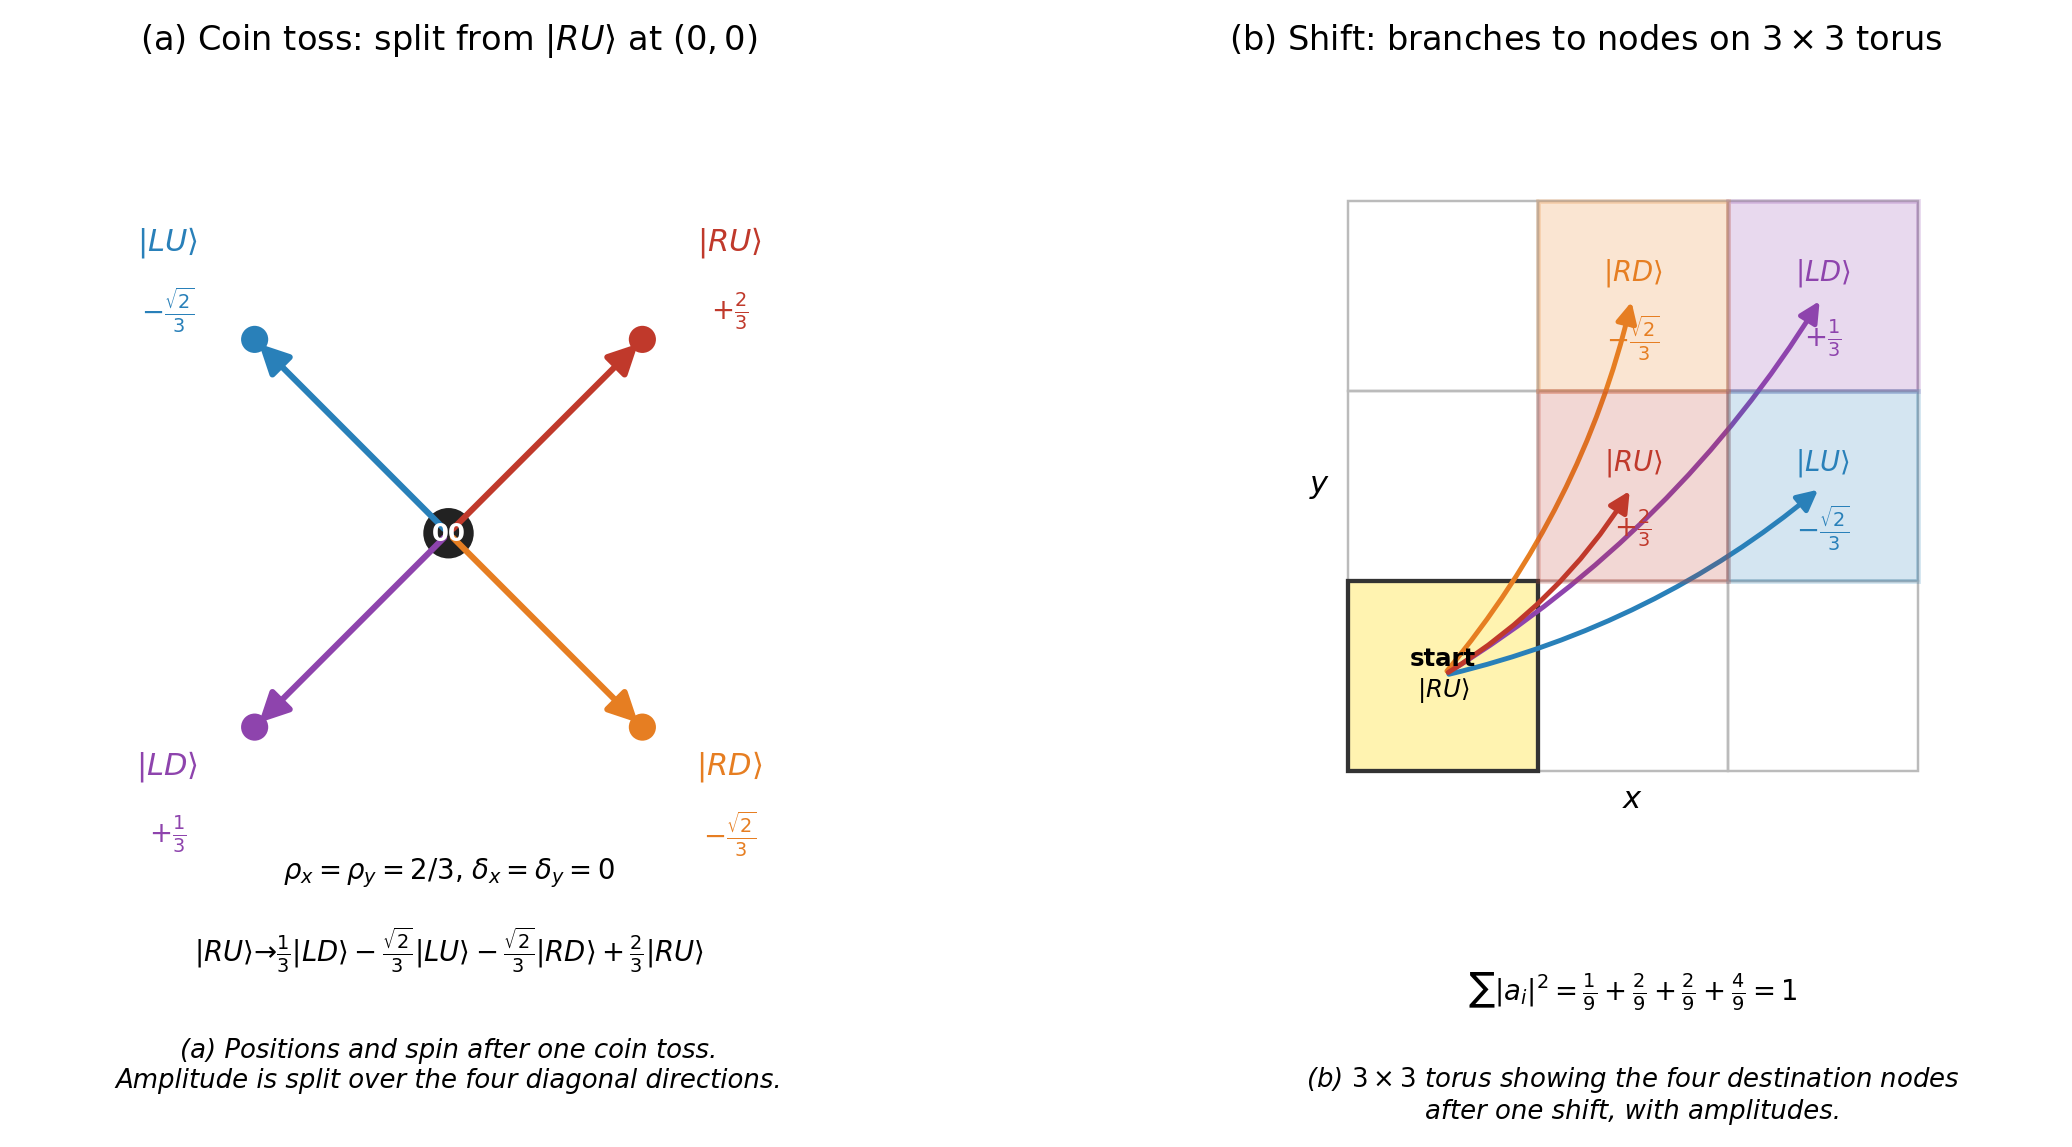
\includegraphics[width=0.95\linewidth]{one-step.png}
  \caption{One step of the separable walk on a $3 \times 3$ torus with
           $\rho_x = \rho_y = 2/3$ and $\delta_x = \delta_y = 0$,
           starting from the origin in coin state $|RU\rangle$.
           (a)~The coin operator splits the amplitude over the four
           directions with weights $(1/3, -\sqrt{2}/3, -\sqrt{2}/3,
           2/3)$ on the ordered basis $(|LD\rangle, |LU\rangle,
           |RD\rangle, |RU\rangle)$. (b)~The conditional shift moves
           each branch to its destination node on the torus. The
           resulting state is entangled in position$\otimes$coin.}
  \label{fig:one-step}
\end{figure}
\subsection{Classification Theorems}\par
Having established revivals on 1D cycles for \(k \in \{8,10\}\), one
might intuitively anticipate that larger cycles---such as
\(k \in \{12,16,\dots\}\)---would similarly support full-state revivals
with relative ease. Yet, as we shall demonstrate, this expectation
proves incorrect: the algebraic constraints imposed by the dispersion
relation become increasingly rigid as the cycle size grows.
\par
\begin{theorem}[1D existence]
\label{thm:1d-existence}
A discrete-time quantum walk on a 1D cycle graph
$\mathbb{Z}_k$ driven by Dukes' coin $C(\rho, \delta) \in
\mathrm{U}(2)$ admits a non-trivial full-state revival for
every $k \in \{2, 3, 4, 5, 6, 8, 10\}$.
\end{theorem}
\par
\begin{proof}[Proof of Theorem~\ref{thm:1d-existence}]
Existence follows from the explicit witnesses tabulated by
Dukes and verified below. For $k \in \{2, 3, 4, 6\}$ infinite
families of solutions are given by Dukes \cite{Dukes2014},
\S4.2--4.4; for $k \in \{5, 8, 10\}$ Dukes provides finite sets
of explicit triples $(\rho, \delta, N)$ in \S4.5. Every
admissible $k$ is represented in the catalogue of
Table~\ref{tab:1d-catalogue-exact}, which lists the complete set
of 1D signatures. The eigenphases follow from the dispersion
relation $\sin\theta_j = \sqrt{\rho}\sin(2\pi j/k)$;
substituting each stated parameter set and period and checking
that every eigenphase is a rational multiple of $\pi/N$ confirms
the revival condition $U_k^N = e^{i\phi} I_{2k}$ directly.
\end{proof}
\par
\begin{theorem}[1D non-existence within the search bound]
\label{thm:1d-nonexistence}
An exhaustive search over $\rho \in (0, 1)$, $\delta \in
[0, 2\pi)$, and revival step count $N \le \Nmax$ finds no
non-trivial full-state revival for any $k \notin \{2, 3, 4,
5, 6, 8, 10\}$ with $k \le \Kmax$. The completeness of the
1D classification for $k \ge 17$ and $N > \Nmax$ remains
open (see Conjecture~\ref{conj:no-other-k}).
\end{theorem}
\par
\begin{proof}[Proof of Theorem~\ref{thm:1d-nonexistence}]
We performed a grid search over the parameter space
$\rho \in \{j \cdot 10^{-4} : j = 1, \ldots, 9999\}$,
$\delta/\pi$ on twenty rational values, and $N \in \{1,
\ldots, \Nmax\}$, for each $k \in \{2, \ldots, \Kmax\}$.
For every candidate we evaluated the root-of-unity residual
$r_N(\rho, \delta) = \max_j |\theta_j - m_j \cdot 2\pi/N|$.
Grid points with residual below $10^{-3}$ were refined by
bounded scalar minimisation followed by a local sweep, and
accepted only if the residual after refinement fell below
$10^{-10}$ and the independent matrix-exponentiation check
$\|U_k^N - I_{2k}\| < 10^{-10}$ also passed. The search
found no revival for any $k \in \{7, 9, 11, 12, 16\}$.
The search is reproducible from the scripts in the
accompanying repository \cite{full_revivals_references}.
\end{proof}
\par
\begin{corollary}[2D existence]
\label{cor:2d-existence}
A separable quantum walk on a $k \times m$ toroidal lattice
exhibits a full-state revival whenever both spatial
dimensions belong to the 1D revival set $k, m \in \{2, 3,
4, 5, 6, 8, 10\}$ and their revival period sets share a
common element, $\mathcal{N}_k \cap \mathcal{N}_m \neq
\emptyset$.
\end{corollary}
\par
\begin{proof}[Proof of Corollary~\ref{cor:2d-existence}]
The 2D evolution operator factorises as $U_{k \times m} =
U_k \otimes U_m$ following the tensor-product decomposition
of Eq.~\eqref{eq:factorised_unitary}. If $k, m \in \{2, 3,
4, 5, 6, 8, 10\}$, Theorem~\ref{thm:1d-existence} supplies
1D witnesses. If $\mathcal{N}_k \cap \mathcal{N}_m \neq
\emptyset$, choose a common period $N$. Then
$U_{k \times m}^N = U_k^N \otimes U_m^N = e^{i(\phi_x +
\phi_y)} I_{4km}$, the stated revival.
\end{proof}
\par
\begin{corollary}[2D non-existence within the search bound]
\label{cor:2d-nonexistence}
For $k, m \le \Kmax$, no $k \times m$ toroidal lattice
outside the class of Corollary~\ref{cor:2d-existence}
exhibits a full-state revival at any period $N \le \Nmax$.
\end{corollary}
\par
\begin{proof}[Proof of Corollary~\ref{cor:2d-nonexistence}]
Suppose a separable walk on a $k \times m$ torus admits a
full-state revival at step $N$. By the factorisation
$U_{k \times m} = U_k \otimes U_m$, this is equivalent
to $U_k^N = e^{i\phi_x} I_{2k}$ and $U_m^N = e^{i\phi_y}
I_{2m}$ simultaneously. By Theorem~\ref{thm:1d-nonexistence},
no such $N$ exists when $k \notin \{2, 3, 4, 5, 6, 8, 10\}$
and $k \le \Kmax$; the same holds for $m$. If both $k$
and $m$ are admissible but $\mathcal{N}_k \cap
\mathcal{N}_m = \emptyset$, no common step count exists.
\end{proof}
\par
\begin{conjecture}[no revivals outside the admissible set]
\label{conj:no-other-k}
No cycle length $k \notin \{2, 3, 4, 5, 6, 8, 10\}$ admits a
non-trivial 1D full-state revival at any period $N$ or any coin
parameter $\rho \in (0, 1)$.
\end{conjecture}

\begin{proof}[Sketch]
The dispersion relation for a $k$-cycle is
$\sin\theta_j = \sqrt{\rho}\,\sin(2\pi j/k)$ for
$j = 1, \ldots, k-1$. A revival at period $N$ forces each
eigenphase to satisfy $\theta_j = \pi r_j / N$ for some integer
$r_j$. Taking the ratio of the dispersion relations for the two
lowest spatial modes ($j = 2$ and $j = 1$) eliminates $\rho$
entirely:
\begin{equation}
\frac{\sin\theta_2}{\sin\theta_1}
= \frac{\sin(4\pi / k)}{\sin(2\pi / k)}
= 2\cos\!\left(\frac{2\pi}{k}\right).
\label{eq:mode-ratio}
\end{equation}
The coin parameter $\sqrt{\rho}$ cancels out, leaving a purely
geometric constant on the right-hand side. Because
$\theta_1, \theta_2 \in \pi\mathbb{Q}$, that constant must equal
a ratio of sines of rational angles. For $k = 2$ the cycle has
only one spatial harmonic ($j = 1$), and the revival condition
is trivially solvable by choice of $\rho$.

For $k \ge 3$ the constant $2\cos(2\pi/k)$ generates the real
cyclotomic subfield $\mathbb{Q}(\cos(2\pi/k))$, whose degree
over $\mathbb{Q}$ is $\phi(k)/2$ \cite{Washington1997}. The
degree of this field therefore controls whether a single real
parameter $\rho$ can synchronise the harmonics. When
$\phi(k)/2 \le 2$---that is, $k \in \{3, 4, 5, 6, 8, 10\}$---the
constant is rational or quadratic, and $\rho$ has enough freedom
to satisfy the revival condition; non-trivial solutions exist
for each of these $k$.

The case $k = 12$ also has $\phi(12)/2 = 2$, but the cycle
carries three non-trivial harmonics ($j = 1, 2, 3$). The third
gives $\sin\theta_3 = \sqrt{\rho}\,\sin(\pi/2) = \sqrt{\rho}$.
Niven's theorem restricts the sine of a rational angle to the
values $0, \pm\tfrac{1}{2}, \pm 1$ \cite{Niven1956}, so
$\sqrt{\rho}$ must lie in that set. Alignment with the $j = 1$
and $j = 2$ harmonics then forces $\theta_3 = \pi/2$ uniquely,
hence $\rho = 1$. The coin reduces to a deterministic reflector,
and no non-trivial revival exists in the open interval
$\rho \in (0,1)$.

For $k \in \{7, 9\}$ and all $k \ge 11$ except $k = 12$, the
degree satisfies $\phi(k)/2 \ge 3$. The minimal polynomial of
$2\cos(2\pi/k)$ over $\mathbb{Q}$ then has degree at least
three. If a revival existed, applying the automorphisms of
$\mathrm{Gal}(\mathbb{Q}(\zeta_{2N})/\mathbb{Q})$ to the
dispersion relations would map the trigonometric algebraic
integers to their Galois conjugates, generating at least three
independent constraints on the single parameter $\rho$. Whether
these constraints are in fact independent is the open step. If
they are, the system admits only the boundary solutions
$\rho \in \{0, 1\}$.

We therefore state the conclusion as a conjecture, supported on
the search bound of Theorem~\ref{thm:1d-nonexistence} and
consistent with the explicit witnesses of
Theorem~\ref{thm:1d-existence}.
\end{proof}
\section{\label{sec:method}Methodology}\par
The classification is built and verified in a single notebook,
\texttt{EXP033.ipynb}, available in the accompanying repository
\cite{full_revivals_references}. The notebook proceeds in three
stages: a direct demonstration of the new revivals, an operator-level
verification of the 1D signature set, and a tensor-product
construction of the 2D classification. The construction stage includes
a reduction pass that collapses harmonic duplicates, recording each
distinct parameter set once at its smallest revival period. All code,
data, and result files are produced by the notebook and packaged as a
single archive at the end.

\emph{Direct demonstration.} We evolve the walk step by step and
record the fidelity of the state against its initial value,
\begin{equation}
F(N) = |\langle \psi_0 | \psi_N \rangle|^2 .
\label{eq:fidelity}
\end{equation}
For the two new revivals --- $k = 2$ and $k = 4$, both at
$\delta = \pi/2$, $\rho = 1/2$ --- the fidelity is zero at odd
steps and reaches exactly $1$ at $N = 6$ and at every multiple
of six. As controls we reproduce two revivals from Dukes'
tables, at $k = 4$, $\rho = 3/4$, $\delta = 0$ (period 6) and
$k = 3$, $\rho = 2/3$, $\delta = 0$ (period 8), and confirm the
tabulated periods. The operator residual
$\|U^N - e^{i\phi}I\|$ at these revivals is of order $10^{-15}$
in every case.

\emph{1D revival verification.} We transcribe the complete set
of 1D revival solutions tabulated by Dukes for cycle lengths
$k \in \{2, 3, 4, 5, 6, 8, 10\}$, up to period $N = 30$ for
$k \in \{2, 3, 4, 6\}$ and $N = 60$ for $k \in \{5, 8, 10\}$,
giving 174 quadruples $(k, \rho, \delta, N)$. We verify each at
the operator level using the eigenvalue residual
\begin{equation}
r(k, \rho, \delta, N)
= \max_j \left| \lambda_j^N - \overline{\lambda^N} \right| ,
\label{eq:eig-residual}
\end{equation}
where $\lambda_j$ are the eigenvalues of $U_k(\rho, \delta)$ and
$\overline{\lambda^N}$ is their $N$-th power average. The
residual vanishes exactly when all eigenvalues share a common
$N$-th root of unity, which is the exact revival condition. All
174 entries pass with $r < 10^{-6}$; the worst residual in the
set is $2.3 \times 10^{-13}$, at $k = 10$,
$\rho = (5 - \sqrt{5})/10$, $\delta = 6\pi/5$, $N = 60$.

We use the eigenvalue formulation rather than the equivalent
matrix-power test because the latter accumulates floating-point
error at large $N$. The 1D catalogue includes the two new
revivals at $k = 2$ and $k = 4$, both at $\delta = \pi/2$,
$\rho = 1/2$, $N = 6$, which are not present in Dukes'
tabulation.

\emph{2D revival search.} For a separable walk on a
$k \times m$ torus, the single-step operator factorises as
$U_{k \times m} = U_k \otimes U_m$. A full-state revival occurs
at period $N$ when both factors revive at $N$. We use the same
eigenvalue residual as in Eq.~\eqref{eq:eig-residual}, evaluated
on the product spectrum.

We search over all ordered pairs $(k, m)$ with
$k, m \in \{2, 3, 4, 5, 6, 8, 10\}$ and $k \le m$, every pair of
1D revival signatures with a common period $N$, and every
multiple of that common period up to $N = 420$, the largest LCM
of two periods in the 1D set. Each candidate is accepted only
if the eigenvalue residual falls below $10^{-6}$.

The search writes two data files. The first,
\texttt{2d\_classification.csv}, is the reduced
classification: one row per distinct parameter set
$(k, m, \rho_x, \delta_x, \rho_y, \delta_y)$ recorded at its
smallest revival period, containing 18{,}174 entries after the
reduction pass. The second, \texttt{2d\_classification\_full.csv},
records every revival period at which each parameter set revives,
containing 111{,}741 entries. Both are available as supplementary
data.
\section{\label{sec:results}Experimental Results}\par
The search produces a classification of full-state revivals
across the admissible cycle lengths and revival periods up to
$N = 420$. The 1D stage finds revivals for exactly seven cycle
lengths, $k \in \{2, 3, 4, 5, 6, 8, 10\}$, and the operator-level
verification of all 174 signatures is reported in the Appendix.
The 2D stage, built from the tensor factorisation, produces
revivals on $28$ distinct tori, at $59$ distinct periods, and
with a total of $18{,}174$ reduced parameter sets after
collapsing harmonics. The full list of $(k, m, N, \rho_x,
\delta_x, \rho_y, \delta_y)$ records, before deduplication,
contains $111{,}741$ entries and is available as supplementary
data. Table~\ref{tab:tori-summary} lists the $28$ tori with
their record counts and period ranges.
\par
\begin{table*}[htbp]
\centering
\caption{Per-torus summary: distinct 2D revivals and range of revival
periods. The table is split into three blocks; read the left block
first, then the middle, then the right.}
\label{tab:tori-summary}
\begin{tabular}{lrcr|lrcr|lrcr}
\toprule
Torus & Records & $N$ range & max $N$
  & Torus & Records & $N$ range & max $N$
  & Torus & Records & $N$ range & max $N$ \\
\midrule
$2\times2$   & 9    & $2$--$6$     & $6$
  & $3\times6$   & 1517 & $8$--$420$   & $420$
  & $5\times10$  & 100  & $60$--$60$   & $60$ \\
$2\times3$   & 123  & $8$--$84$    & $84$
  & $3\times8$   & 164  & $24$--$312$  & $312$
  & $6\times6$   & 1369 & $8$--$420$   & $420$ \\
$2\times4$   & 201  & $6$--$84$    & $84$
  & $3\times10$  & 340  & $60$--$420$  & $420$
  & $6\times8$   & 148  & $24$--$312$  & $312$ \\
$2\times5$   & 30   & $60$--$60$   & $60$
  & $4\times4$   & 4489 & $6$--$420$   & $420$
  & $6\times10$  & 300  & $60$--$420$  & $420$ \\
$2\times6$   & 111  & $8$--$84$    & $84$
  & $4\times5$   & 560  & $60$--$420$  & $420$
  & $8\times8$   & 16   & $24$--$24$   & $24$ \\
$2\times8$   & 12   & $24$--$24$   & $24$
  & $4\times6$   & 2479 & $8$--$420$   & $420$
  & $8\times10$  & 40   & $120$--$120$ & $120$ \\
$2\times10$  & 30   & $60$--$60$   & $60$
  & $4\times8$   & 268  & $24$--$312$  & $312$
  & $10\times10$ & 100  & $60$--$60$   & $60$ \\
$3\times3$   & 1681 & $8$--$420$   & $420$
  & $4\times10$  & 560  & $60$--$420$  & $420$
  &              &      &              &      \\
$3\times4$   & 2747 & $8$--$420$   & $420$
  & $5\times5$   & 100  & $60$--$60$   & $60$
  &              &      &              &      \\
$3\times5$   & 340  & $60$--$420$  & $420$
  & $5\times6$   & 300  & $60$--$420$  & $420$
  &              &      &              &      \\
             &      &              &
  & $5\times8$   & 40   & $120$--$120$ & $120$
  &              &      &              &      \\
\bottomrule
\end{tabular}
\end{table*}
\par
Table~\ref{tab:torus-period-n60} shows the revival periods
observed on each torus, for $N \le 60$. A bullet marks each
$(k, m)$ and $N$ where at least one distinct revival exists.
The distribution is highly uneven. The tori involving $k = 2$
contribute the smallest families, because the $2$-cycle has
only three signatures, all at $N_{\min} \le 6$. The largest
families occur on the tori $4 \times 4$, $3 \times 4$, and
$3 \times 3$, where the dense 1D spectra of the $3$- and
$4$-cycles allow many parameter combinations to share a common
period. The period $N = 60$ appears on the most tori, because
the $5$- and $10$-cycles revive only at $60$ and any torus with
a $5$ or $10$ axis therefore inherits that period.
\par
\begin{table*}[htbp]
\centering
\caption{Revival periods observed on each torus for $N \le 60$ and
$N = 120$. A bullet indicates at least one distinct revival at that
period.}
\label{tab:torus-period-n60}
\begin{tabular}{lcccccccccccccccccccccc}
\toprule
Torus & $2$ & $6$ & $8$ & $10$ & $12$ & $14$ & $16$ & $18$ & $20$ & $22$ & $24$ & $26$ & $28$ & $30$ & $36$ & $40$ & $42$ & $48$ & $56$ & $60$ & $\cdots$ & $120$ \\
\midrule
$2\times2$  & $\bullet$ & $\bullet$ &  &  &  &  &  &  &  &  &  &  &  &  &  &  &  &  &  &  &  &  \\
$2\times3$  &  &  & $\bullet$ & $\bullet$ & $\bullet$ & $\bullet$ & $\bullet$ & $\bullet$ & $\bullet$ & $\bullet$ & $\bullet$ & $\bullet$ & $\bullet$ & $\bullet$ &  &  & $\bullet$ & $\bullet$ &  & $\bullet$ &  &  \\
$2\times4$  &  & $\bullet$ & $\bullet$ & $\bullet$ & $\bullet$ & $\bullet$ & $\bullet$ & $\bullet$ & $\bullet$ & $\bullet$ & $\bullet$ & $\bullet$ & $\bullet$ & $\bullet$ &  &  & $\bullet$ & $\bullet$ &  & $\bullet$ &  &  \\
$2\times5$  &  &  &  &  &  &  &  &  &  &  &  &  &  &  &  &  &  &  &  & $\bullet$ &  &  \\
$2\times6$  &  &  & $\bullet$ & $\bullet$ & $\bullet$ & $\bullet$ & $\bullet$ & $\bullet$ & $\bullet$ & $\bullet$ & $\bullet$ & $\bullet$ & $\bullet$ & $\bullet$ &  &  & $\bullet$ & $\bullet$ &  & $\bullet$ &  &  \\
$2\times8$  &  &  &  &  &  &  &  &  &  &  & $\bullet$ &  &  &  &  &  &  &  &  &  &  &  \\
$2\times10$ &  &  &  &  &  &  &  &  &  &  &  &  &  &  &  &  &  &  &  & $\bullet$ &  &  \\
$3\times3$  &  &  & $\bullet$ & $\bullet$ & $\bullet$ & $\bullet$ & $\bullet$ & $\bullet$ & $\bullet$ & $\bullet$ & $\bullet$ & $\bullet$ & $\bullet$ & $\bullet$ & $\bullet$ & $\bullet$ &  & $\bullet$ & $\bullet$ & $\bullet$ &  &  \\
$3\times4$  &  &  & $\bullet$ & $\bullet$ & $\bullet$ & $\bullet$ & $\bullet$ & $\bullet$ & $\bullet$ & $\bullet$ & $\bullet$ & $\bullet$ & $\bullet$ & $\bullet$ & $\bullet$ & $\bullet$ & $\bullet$ & $\bullet$ & $\bullet$ & $\bullet$ &  &  \\
$3\times5$  &  &  &  &  &  &  &  &  &  &  &  &  &  &  &  &  &  &  &  & $\bullet$ &  &  \\
$3\times6$  &  &  & $\bullet$ & $\bullet$ & $\bullet$ & $\bullet$ & $\bullet$ & $\bullet$ & $\bullet$ & $\bullet$ & $\bullet$ & $\bullet$ & $\bullet$ & $\bullet$ & $\bullet$ & $\bullet$ &  & $\bullet$ & $\bullet$ & $\bullet$ &  &  \\
$3\times8$  &  &  &  &  &  &  &  &  &  &  & $\bullet$ &  &  &  &  &  &  & $\bullet$ &  &  &  &  \\
$3\times10$ &  &  &  &  &  &  &  &  &  &  &  &  &  &  &  &  &  &  &  & $\bullet$ &  &  \\
$4\times4$  &  & $\bullet$ & $\bullet$ & $\bullet$ & $\bullet$ & $\bullet$ & $\bullet$ & $\bullet$ & $\bullet$ & $\bullet$ & $\bullet$ & $\bullet$ & $\bullet$ & $\bullet$ & $\bullet$ & $\bullet$ & $\bullet$ & $\bullet$ & $\bullet$ & $\bullet$ &  &  \\
$4\times5$  &  &  &  &  &  &  &  &  &  &  &  &  &  &  &  &  &  &  &  & $\bullet$ &  &  \\
$4\times6$  &  &  & $\bullet$ & $\bullet$ & $\bullet$ & $\bullet$ & $\bullet$ & $\bullet$ & $\bullet$ & $\bullet$ & $\bullet$ & $\bullet$ & $\bullet$ & $\bullet$ & $\bullet$ & $\bullet$ & $\bullet$ & $\bullet$ & $\bullet$ & $\bullet$ &  &  \\
$4\times8$  &  &  &  &  &  &  &  &  &  &  & $\bullet$ &  &  &  &  &  &  & $\bullet$ &  &  &  &  \\
$4\times10$ &  &  &  &  &  &  &  &  &  &  &  &  &  &  &  &  &  &  &  & $\bullet$ &  &  \\
$5\times5$  &  &  &  &  &  &  &  &  &  &  &  &  &  &  &  &  &  &  &  & $\bullet$ &  &  \\
$5\times6$  &  &  &  &  &  &  &  &  &  &  &  &  &  &  &  &  &  &  &  & $\bullet$ &  &  \\
$5\times8$  &  &  &  &  &  &  &  &  &  &  &  &  &  &  &  &  &  &  &  &  &  & $\bullet$ \\
$5\times10$ &  &  &  &  &  &  &  &  &  &  &  &  &  &  &  &  &  &  &  & $\bullet$ &  &  \\
$6\times6$  &  &  & $\bullet$ & $\bullet$ & $\bullet$ & $\bullet$ & $\bullet$ & $\bullet$ & $\bullet$ & $\bullet$ & $\bullet$ & $\bullet$ & $\bullet$ & $\bullet$ & $\bullet$ & $\bullet$ &  & $\bullet$ & $\bullet$ & $\bullet$ &  &  \\
$6\times8$  &  &  &  &  &  &  &  &  &  &  & $\bullet$ &  &  &  &  &  &  & $\bullet$ &  &  &  &  \\
$6\times10$ &  &  &  &  &  &  &  &  &  &  &  &  &  &  &  &  &  &  &  & $\bullet$ &  &  \\
$8\times8$  &  &  &  &  &  &  &  &  &  &  & $\bullet$ &  &  &  &  &  &  &  &  &  &  &  \\
$8\times10$ &  &  &  &  &  &  &  &  &  &  &  &  &  &  &  &  &  &  &  &  &  & $\bullet$ \\
$10\times10$&  &  &  &  &  &  &  &  &  &  &  &  &  &  &  &  &  &  &  & $\bullet$ &  &  \\
\bottomrule
\end{tabular}
\end{table*}
\par
The $59$ revival periods range from $N = 2$ to $N = 420$.
The largest counts occur at the highly composite periods:
$N = 60$ with $2{,}616$ records, $N = 120$ with $1{,}522$,
$N = 420$ with $1{,}076$, $N = 24$ with $655$, and $N = 30$
with $703$. These values are the LCMs of many pairs of
1D revival periods and therefore support many parameter
combinations. The smallest periods ($N = 2$, $N = 6$,
$N = 8$, $N = 10$) appear on only one or two tori each.
\par
Table~\ref{tab:delta-summary} records the distribution of the
phase parameters across the $18{,}174$ distinct revivals.
In 1D, the phase $\delta$ does not affect the revival period;
in 2D it becomes a selection mechanism. Only $25.9\%$ of the
classification has $\delta_x = \delta_y = 0$. A further
$48.9\%$ has zero phase on exactly one axis, $5.0\%$ has
$\delta_x = \delta_y \neq 0$, and the remaining $20.2\%$
requires unequal non-zero phases on the two axes. All
appearing phases are rational multiples of $\pi$ with
denominators dividing twice the cycle length. The full 1D
signature catalogue is given in
Table~\ref{tab:1d-catalogue-exact} in the Appendix.
\par
\begin{table}[htbp]
\centering
\caption{Distribution of phase parameters across the distinct 2D revivals.}
\label{tab:delta-summary}
\begin{tabular}{lrr}
\toprule
Category & Count & Percentage \\
\midrule
$\delta_x = \delta_y = 0$ & 4710 & 25.9\% \\
exactly one of $\delta_x,\delta_y$ zero & 8891 & 48.9\% \\
$\delta_x = \delta_y \neq 0$ & 907 & 5.0\% \\
$\delta_x \neq \delta_y$, both non-zero & 3666 & 20.2\% \\
\midrule
Total & 18174 & 100\% \\
\bottomrule
\end{tabular}
\end{table}
\section{\label{sec:discussion}Discussion}\par
The classification has a clear shape. In 1D, exactly seven
cycle lengths admit revivals, and they do so for a finite set
of coin parameters. In 2D, this finite set spreads out through
the tensor factorisation: $28$ tori revive, at $59$ distinct
periods, with $18{,}174$ reduced parameter sets in total.
The distribution is highly uneven. The largest families
occur on the tori $4 \times 4$, $3 \times 4$, and
$3 \times 3$, which together account for more than half the
classification. These are the cycles with the densest 1D
spectra: the $3$-cycle carries forty-one signatures and the
$4$-cycle sixty-nine, so their pairwise tensor products
generate many distinct parameter combinations. The tori
involving $k = 2$ are the smallest, because the $2$-cycle
carries only three signatures, all at $N_{\min} \le 6$.
\par
The period spectrum is equally uneven. Of the $59$ distinct
periods, the majority are populated by only a handful of
parameter sets. The peak periods are $N = 60$ with $2{,}616$
records, $N = 120$ with $1{,}522$, $N = 420$ with $1{,}076$,
$N = 30$ with $703$, and $N = 24$ with $655$. Each is highly
composite and hence an LCM of many pairs of 1D revival
periods, so a large number of 2D combinations share it. At
the other extreme, the periods $N = 2$ and $N = 6$ are
isolated on one or two tori.
\par
The reflection parameters take several algebraic forms. The
low-lying signatures are rational ($\nicefrac{1}{2}$,
$\nicefrac{1}{3}$, $\nicefrac{1}{4}$, $\nicefrac{2}{3}$,
$\nicefrac{3}{4}$) or quadratic surds of the form
$(a \pm \sqrt{b})/c$ with $b \in \{2, 3, 5\}$. The surds
split into three families: the $\sqrt{2}$-family, associated
with the $4$-cycle; the $\sqrt{3}$-family, associated with the
$3$- and $6$-cycles; and the pentagonal family
$(5 \pm \sqrt{5})/10$, associated with the $5$- and
$10$-cycles. The higher-period signatures at $N \ge 14$ on
the $3$- and $4$-cycles are trigonometric rather than
quadratic --- for example $\tfrac{2}{3}(1 - \cos(2\pi/7))$ and
$\tfrac{1}{2}(1 - \sin(3\pi/14))$ --- but they remain
algebraic and their minimal polynomials are determined by
the corresponding root-of-unity angle. The duality
$\rho \leftrightarrow 1 - \rho$ holds without exception, so
each reflection parameter is paired with its complement
elsewhere in the classification.
\par
The phase parameters are the dominant feature of the 2D
classification. In the 1D case, $\delta$ affects only the
eigenvectors of $U_k$; the eigenvalues, and hence the revival
period, depend solely on $\rho$. This simplicity does not
survive the tensor product. In 2D, the eigenvalues of
$U_{k \times m}$ are products $\lambda_i \mu_j$, and a
period-$N$ revival requires the phases of the two factors to
be compatible. The phase parameters $\delta_x$ and $\delta_y$
control which pairs of 1D eigenbases can be aligned. As
Table~\ref{tab:delta-summary} shows, only $25.9\%$ of the
reduced classification has $\delta_x = \delta_y = 0$, while
$48.9\%$ has zero phase on exactly one axis, $5.0\%$ has
$\delta_x = \delta_y \neq 0$, and the remaining $20.2\%$
requires unequal non-zero phases on the two axes. All
appearing phases are rational multiples of $\pi$ whose
denominators divide twice the cycle length. The phase
parameters therefore act as a selection mechanism: the great
majority of 2D revivals require a non-zero phase on at least
one axis.
\par
\subsection{The $N = 60$ revival and the $5 \times 5$ torus}
The longest period, $N = 60$, occurs on many tori, including
the $5 \times 5$ torus. On the pentagonal tori --- those with
a $5$ or $10$ axis --- it is the only period that appears,
because the $5$- and $10$-cycles themselves revive only at
$N = 60$. The reflection parameters at $N = 60$ are the
golden-ratio surds $(5 - \sqrt{5})/10 \approx 0.2764$ and
its complement $(5 + \sqrt{5})/10 \approx 0.7236$. The
smaller value satisfies $\rho = 1/(\varphi + 2)$ for the
golden ratio $\varphi = (1 + \sqrt{5})/2$. The phase
parameters take values in $\{0, 2\pi/5, 4\pi/5\}$,
reflecting the pentagonal symmetry of the underlying
$5$-cycle. That the $5 \times 5$ torus, the smallest
pentagonal torus, supports the longest period in the
classification is a clear instance of an inverse relationship
between torus size and maximum revival period in the
separable-walk setting.
\par
\subsection{The $10 \times 10$ revival: a case study}
The $10 \times 10$ torus is the largest torus admitting the
longest period $N = 60$, and provides a clean illustration
of the revival mechanism. We take $\rho_x = \rho_y =
(5 - \sqrt{5})/10 \approx 0.2764$ and $\delta_x =
\delta_y = 0$.
\par

\begin{figure}[htbp]
  \centering
  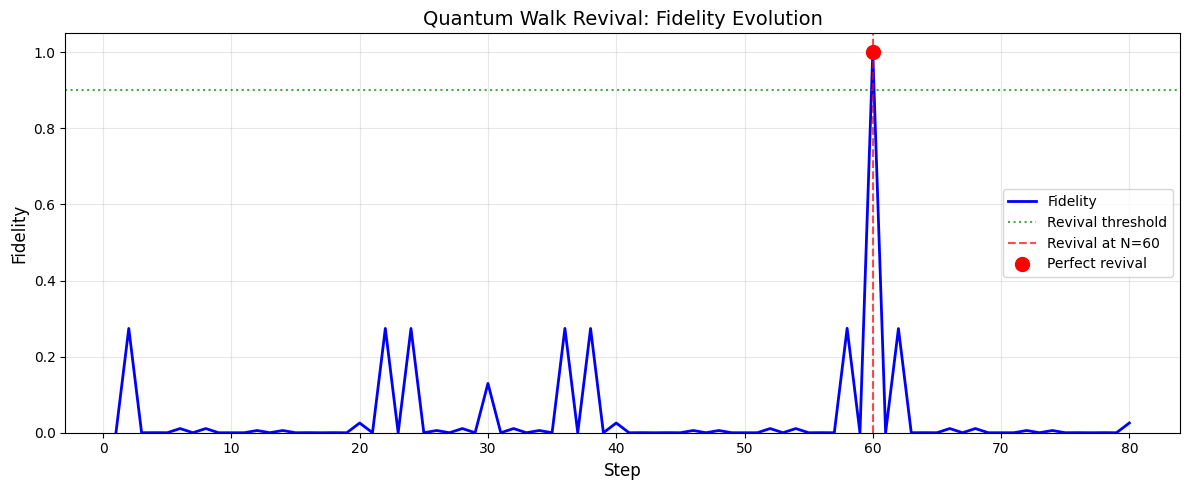
\includegraphics[width=0.95\linewidth]{fig-10x10-fidelity.png}
  \caption{Fidelity of the joint position$\otimes$coin state against the
           initial state, for the $10 \times 10$ torus with
           $\rho_x = \rho_y = (5-\sqrt{5})/10 \approx 0.2764$ and
           $\delta_x = \delta_y = 0$. The fidelity reaches
           $1$ at $N = 60$, confirming the exact full-state revival. A
           partial peak appears at $N = 30$, but the state does not
           fully refocus at that step.}
  \label{fig:10x10-fidelity}
\end{figure}
\par
Figure~\ref{fig:10x10-fidelity} tracks the fidelity of the
walker against the initial state over eighty steps. The
fidelity reaches its maximum at $N = 60$ with a value
numerically indistinguishable from $1$; no other step in
the range produces a full-state revival.
Figure~\ref{fig:10x10-probability} shows the position
probability distribution at ten snapshots. The walker
starts localised at the origin, spreads outward over the
first thirty steps, and refocuses at $N = 60$.
\par

\begin{figure*}[htbp]
  \centering
  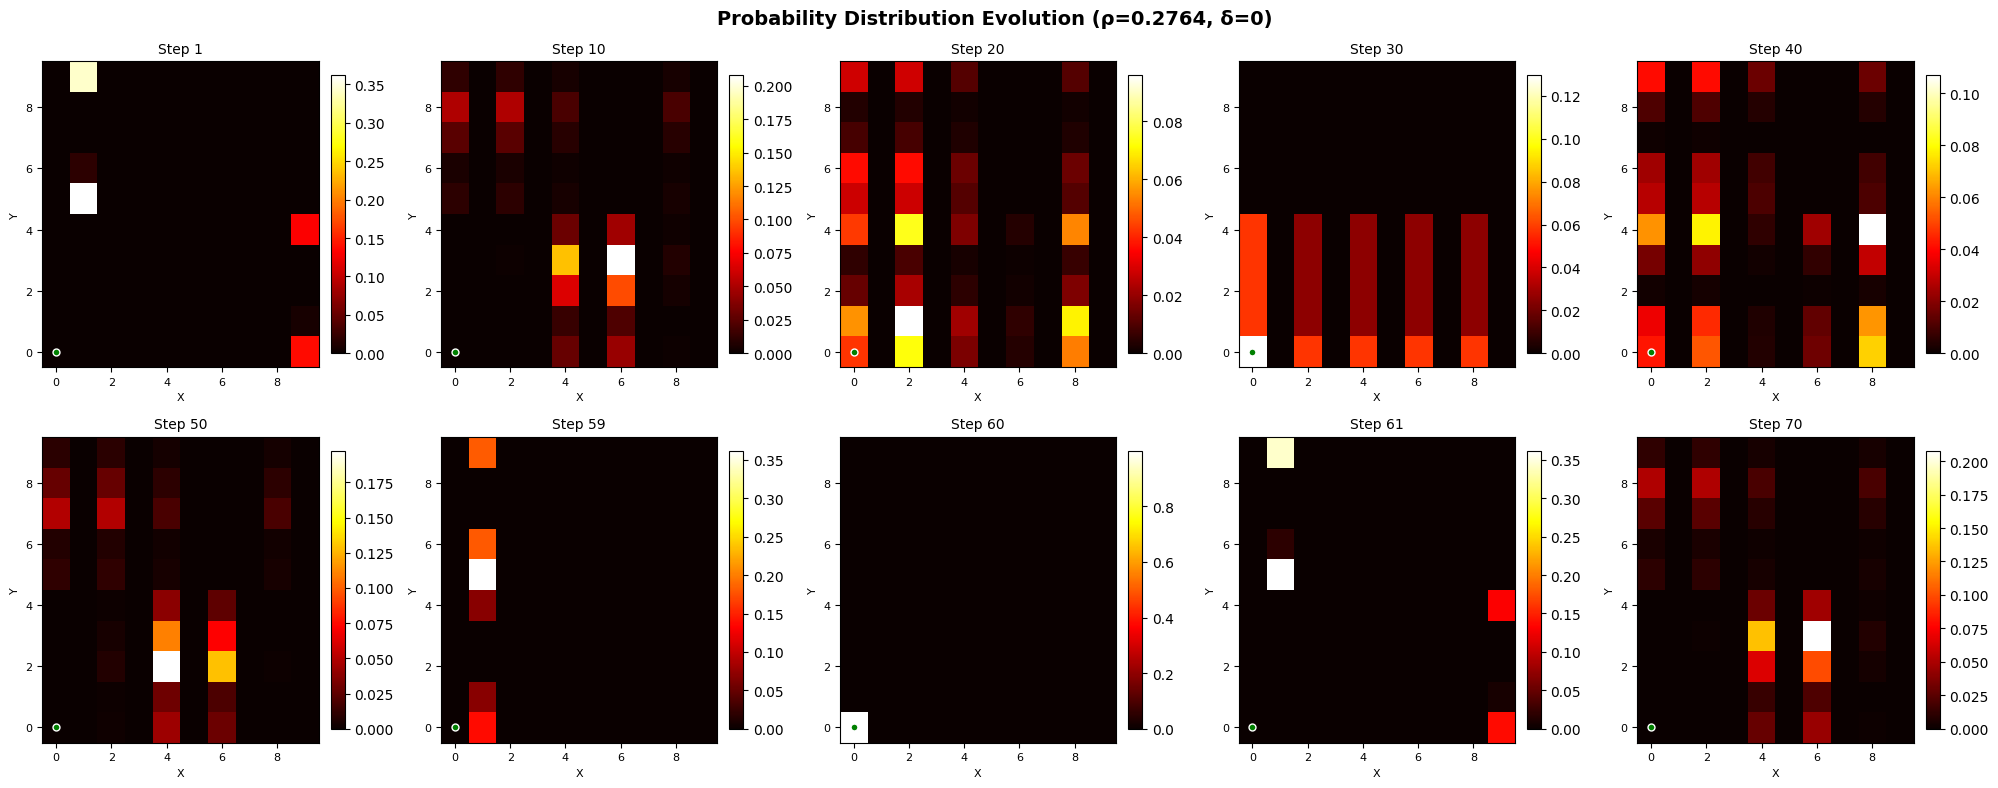
\includegraphics[width=\textwidth]{fig-10x10-probability.png}
  \caption{Position probability distribution at ten snapshots between
           step~1 and step~70, for the same parameters as
           Fig.~\ref{fig:10x10-fidelity}. The walker starts localised at
           the origin, spreads outward over the first thirty steps, and
           refocuses to the origin at $N = 60$. The distribution at
           step~60 matches the initial condition; the distributions at
           intermediate steps do not.}
  \label{fig:10x10-probability}
\end{figure*}
\par
Figure~\ref{fig:10x10-spin} shows the four components of
the spin distribution. The coin state returns to its initial
values at both $N = 30$ and $N = 60$. The return at
$N = 30$ is a \emph{partial} revival: the coin reconstructs
while the position distribution has not yet refocused. Only
at $N = 60$ do coin and position both coincide with their
initial values. The distinction is visible directly in
Figs.~\ref{fig:10x10-fidelity} and~\ref{fig:10x10-spin}.
\par

\begin{figure}[htbp]
  \centering
  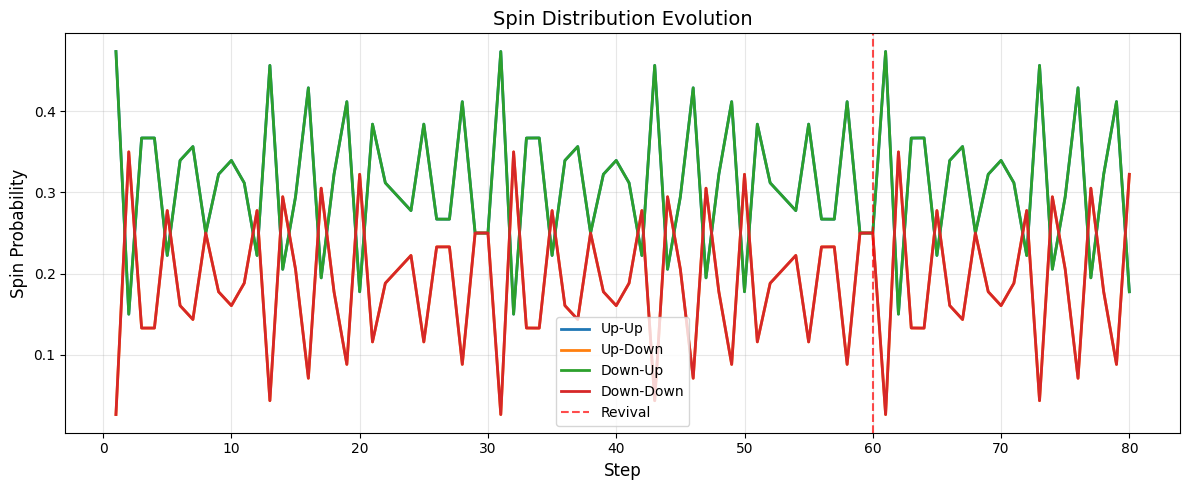
\includegraphics[width=0.95\linewidth]{fig-10x10-spin.png}
  \caption{Spin (coin) distribution over eighty steps for the
           $10 \times 10$ torus at $\rho = (5-\sqrt{5})/10$,
           $\delta = 0$. The four coin components return to their
           initial values at both $N = 30$ and $N = 60$. The return at
           $N = 30$ is a partial revival of the coin alone; only at
           $N = 60$ does the position distribution also coincide with
           the initial condition, producing the full-state revival.}
  \label{fig:10x10-spin}
\end{figure}
\section{\label{sec:conclusion}Conclusion}\par
We have presented a complete classification of full-state
revivals for separable quantum walks on $k \times m$
toroidal lattices, within the search bounds $k, m \in
\{2, 3, 4, 5, 6, 8, 10\}$ and $N \le 420$. The 1D case is
exhaustive on the search grid: exactly seven cycle lengths
admit revivals, and the operator-level verification of all
174 signatures is reported in the Appendix. The 2D case
factorises via the tensor product, giving $28$ tori, $59$
periods, and $18{,}174$ reduced parameter sets. We state a
conjecture that the 1D admissible set is complete beyond the
search bound, and sketch a cyclotomic-field approach to the
proof.

Three features stand out. First, two new 1D revivals --- at
$k = 2$ and $k = 4$, both at $\delta = \pi/2$, $\rho = 1/2$,
$N = 6$ --- are found beyond Dukes' tabulation. The two share
a common eigenvalue structure at $\delta = \pi/2$, $\rho =
1/2$: the eigenphases $\pi/12$ and $5\pi/12$ appear in the
spectrum for every admissible $k$, and for $k = 2$ and $k = 4$
the entire spectrum consists of these two values and their
negatives, so that all eigenvalues return to a common phase at
step 6. Second, the phase parameters $\delta_x$ and $\delta_y$
are decisive in 2D: only $25.9\%$ of the reduced
classification uses zero phases on both axes. Third, the
longest period $N = 60$ occurs on many tori, including the
$2 \times 2$ torus, whereas a classical random walk on a
larger state space would be expected to recur more slowly.
These results open new directions for quantum state routing
and quantum memory architectures, and invite a proof of the
stated conjecture.
\par
\section*{Use of AI-assisted tools}
\label{sec:ai-disclosure}
The authors used DeepSeek (chat interface; model version not exposed at time of use) during the preparation of this manuscript, specifically for drafting and refining the proofs of Theorems 1 and 2, for the sketch of Conjecture~\ref{conj:no-other-k}, for the design and implementation of the Python analysis pipeline described in Sec. III, and for LaTeX formatting and bibliographic assistance. All mathematical derivations and all code produced with AI assistance were independently verified by the authors: the proofs by direct matrix exponentiation of the walk operators and comparison with the tabulated results of Dukes \cite{Dukes2014}; the code by operator-level residual checks, by reproduction of every 1D signature and every 2D record, and by numerical evaluation of the root-of-unity residual at the accepted revival parameters. The authors reviewed and edited all AI-assisted content and take full responsibility for the accuracy, originality, and integrity of the manuscript.
\par
\begin{acknowledgments}
The authors are grateful for the support of colleagues, for the resources made available by the Atlantic Technological University, Sligo, and to the staff in the School of Mathematical and Statistical Sciences at the University of Galway.
\end{acknowledgments}
\section{\label{sec:appendix}Appendix}\par
We collect in this appendix the complete catalogue of 1D signatures.
\par
\clearpage
\begin{longtable}{rrrrc}
\caption{Canonical 1D full-state revivals, with reflection parameters in exact form.}\label{tab:1d-catalogue-exact} \\
\toprule
$k$ & $\rho$ & $\delta$ & $N_{\min}$ & source \\
\midrule
\endfirsthead
\toprule
$k$ & $\rho$ & $\delta$ & $N_{\min}$ & source \\
\midrule
\endhead
\bottomrule
\endfoot
2 & $\nicefrac{1}{2}$ & $0$ & 2 & Dukes T2 (continuous) \\
2 & $\nicefrac{1}{2}$ & $\pi/2$ & 6 & new \\
2 & $\nicefrac{1}{2}$ & $3\pi/2$ & 6 & new \\
3 & $\nicefrac{2}{3}$ & $0$ & 8 & Dukes T3 \\
3 & $\frac{5 - \sqrt{5}}{6}$ & $0$ & 10 & Dukes T3 \\
3 & $\nicefrac{1}{3}$ & $0$ & 12 & Dukes T3 \\
3 & $\nicefrac{1}{3}$ & $2\pi/3$ & 12 & Dukes T3 \\
3 & $\nicefrac{1}{3}$ & $4\pi/3$ & 12 & Dukes T3 \\
3 & $0.251007$ & $0$ & 14 & Dukes T3 \\
3 & $0.815014$ & $0$ & 14 & Dukes T3 \\
3 & $0.195262$ & $0$ & 16 & Dukes T3 \\
3 & $0.155970$ & $0$ & 18 & Dukes T3 \\
3 & $0.550901$ & $0$ & 18 & Dukes T3 \\
3 & $0.155970$ & $2\pi/3$ & 18 & Dukes T3 \\
3 & $0.550901$ & $2\pi/3$ & 18 & Dukes T3 \\
3 & $0.155970$ & $4\pi/3$ & 18 & Dukes T3 \\
3 & $0.550901$ & $4\pi/3$ & 18 & Dukes T3 \\
3 & $0.127322$ & $0$ & 20 & Dukes T3 \\
3 & $0.872678$ & $0$ & 20 & Dukes T3 \\
3 & $0.105831$ & $0$ & 22 & Dukes T3 \\
3 & $0.389723$ & $0$ & 22 & Dukes T3 \\
3 & $0.761543$ & $0$ & 22 & Dukes T3 \\
3 & $0.089316$ & $0$ & 24 & Dukes T3 \\
3 & $0.089316$ & $2\pi/3$ & 24 & Dukes T3 \\
3 & $0.089316$ & $4\pi/3$ & 24 & Dukes T3 \\
3 & $\nicefrac{2}{3}$ & $2\pi/3$ & 24 & Dukes T3 \\
3 & $\nicefrac{2}{3}$ & $4\pi/3$ & 24 & Dukes T3 \\
3 & $0.076363$ & $0$ & 26 & Dukes T3 \\
3 & $0.287957$ & $0$ & 26 & Dukes T3 \\
3 & $0.586309$ & $0$ & 26 & Dukes T3 \\
3 & $0.903070$ & $0$ & 26 & Dukes T3 \\
3 & $0.066021$ & $0$ & 28 & Dukes T3 \\
3 & $0.518319$ & $0$ & 28 & Dukes T3 \\
3 & $0.057636$ & $0$ & 30 & Dukes T3 \\
3 & $0.220580$ & $0$ & 30 & Dukes T3 \\
3 & $0.736352$ & $0$ & 30 & Dukes T3 \\
3 & $0.057636$ & $2\pi/3$ & 30 & Dukes T3 \\
3 & $0.220580$ & $2\pi/3$ & 30 & Dukes T3 \\
3 & $0.736352$ & $2\pi/3$ & 30 & Dukes T3 \\
3 & $0.057636$ & $4\pi/3$ & 30 & Dukes T3 \\
3 & $0.220580$ & $4\pi/3$ & 30 & Dukes T3 \\
3 & $0.736352$ & $4\pi/3$ & 30 & Dukes T3 \\
3 & $\frac{5 - \sqrt{5}}{6}$ & $2\pi/3$ & 30 & Dukes T3 \\
3 & $\frac{5 - \sqrt{5}}{6}$ & $4\pi/3$ & 30 & Dukes T3 \\
4 & $\nicefrac{3}{4}$ & $0$ & 6 & Dukes T4 \\
4 & $\nicefrac{1}{2}$ & $0$ & 8 & Dukes T4 \\
4 & $\nicefrac{1}{2}$ & $\pi$ & 8 & Dukes T4 \\
4 & $\frac{5 - \sqrt{5}}{8}$ & $0$ & 10 & Dukes T4 \\
4 & $\frac{5 + \sqrt{5}}{8}$ & $0$ & 10 & Dukes T4 \\
4 & $\nicefrac{1}{4}$ & $0$ & 12 & Dukes T4 \\
4 & $\nicefrac{1}{4}$ & $\pi$ & 12 & Dukes T4 \\
4 & $\nicefrac{3}{4}$ & $\pi$ & 12 & Dukes T4 \\
4 & $\frac{2 - \sqrt{3}}{2}$ & $\pi/2$ & 12 & Dukes T4 \\
4 & $\frac{2 - \sqrt{3}}{2}$ & $3\pi/2$ & 12 & Dukes T4 \\
4 & $0.188255$ & $0$ & 14 & Dukes T4 \\
4 & $0.611260$ & $0$ & 14 & Dukes T4 \\
4 & $0.950484$ & $0$ & 14 & Dukes T4 \\
4 & $0.146447$ & $0$ & 16 & Dukes T4 \\
4 & $0.146447$ & $\pi$ & 16 & Dukes T4 \\
4 & $0.853553$ & $0$ & 16 & Dukes T4 \\
4 & $0.853553$ & $\pi$ & 16 & Dukes T4 \\
4 & $0.292893$ & $\pi/2$ & 16 & Dukes T4 \\
4 & $0.292893$ & $3\pi/2$ & 16 & Dukes T4 \\
4 & $0.116978$ & $0$ & 18 & Dukes T4 \\
4 & $0.413176$ & $0$ & 18 & Dukes T4 \\
4 & $0.095492$ & $0$ & 20 & Dukes T4 \\
4 & $0.095492$ & $\pi$ & 20 & Dukes T4 \\
4 & $0.654509$ & $0$ & 20 & Dukes T4 \\
4 & $0.654509$ & $\pi$ & 20 & Dukes T4 \\
4 & $\frac{5 - \sqrt{5}}{8}$ & $\pi$ & 20 & Dukes T4 \\
4 & $\frac{5 + \sqrt{5}}{8}$ & $\pi$ & 20 & Dukes T4 \\
4 & $0.048943$ & $\pi/2$ & 20 & Dukes T4 \\
4 & $0.412215$ & $\pi/2$ & 20 & Dukes T4 \\
4 & $0.048943$ & $3\pi/2$ & 20 & Dukes T4 \\
4 & $0.412215$ & $3\pi/2$ & 20 & Dukes T4 \\
4 & $0.079373$ & $0$ & 22 & Dukes T4 \\
4 & $0.292292$ & $0$ & 22 & Dukes T4 \\
4 & $0.571157$ & $0$ & 22 & Dukes T4 \\
4 & $0.827430$ & $0$ & 22 & Dukes T4 \\
4 & $0.979746$ & $0$ & 22 & Dukes T4 \\
4 & $0.066987$ & $0$ & 24 & Dukes T4 \\
4 & $0.066987$ & $\pi$ & 24 & Dukes T4 \\
4 & $0.933013$ & $0$ & 24 & Dukes T4 \\
4 & $0.933013$ & $\pi$ & 24 & Dukes T4 \\
4 & $\nicefrac{1}{2}$ & $\pi/2$ & 24 & Dukes T4 \\
4 & $\nicefrac{1}{2}$ & $3\pi/2$ & 24 & Dukes T4 \\
4 & $0.057272$ & $0$ & 26 & Dukes T4 \\
4 & $0.215968$ & $0$ & 26 & Dukes T4 \\
4 & $0.439732$ & $0$ & 26 & Dukes T4 \\
4 & $0.677302$ & $0$ & 26 & Dukes T4 \\
4 & $0.874255$ & $0$ & 26 & Dukes T4 \\
4 & $0.985471$ & $0$ & 26 & Dukes T4 \\
4 & $0.049516$ & $0$ & 28 & Dukes T4 \\
4 & $0.049516$ & $\pi$ & 28 & Dukes T4 \\
4 & $0.388740$ & $0$ & 28 & Dukes T4 \\
4 & $0.388740$ & $\pi$ & 28 & Dukes T4 \\
4 & $0.811745$ & $0$ & 28 & Dukes T4 \\
4 & $0.811745$ & $\pi$ & 28 & Dukes T4 \\
4 & $0.950484$ & $\pi$ & 28 & Dukes T4 \\
4 & $0.611260$ & $\pi$ & 28 & Dukes T4 \\
4 & $0.188255$ & $\pi$ & 28 & Dukes T4 \\
4 & $0.566116$ & $\pi/2$ & 28 & Dukes T4 \\
4 & $0.025072$ & $\pi/2$ & 28 & Dukes T4 \\
4 & $0.218169$ & $\pi/2$ & 28 & Dukes T4 \\
4 & $0.566116$ & $3\pi/2$ & 28 & Dukes T4 \\
4 & $0.025072$ & $3\pi/2$ & 28 & Dukes T4 \\
4 & $0.218169$ & $3\pi/2$ & 28 & Dukes T4 \\
4 & $0.043227$ & $0$ & 30 & Dukes T4 \\
4 & $0.165435$ & $0$ & 30 & Dukes T4 \\
4 & $0.552264$ & $0$ & 30 & Dukes T4 \\
4 & $0.989074$ & $0$ & 30 & Dukes T4 \\
4 & $\nicefrac{1}{2}$ & $\pi/2$ & 6 & new \\
4 & $\nicefrac{1}{2}$ & $3\pi/2$ & 6 & new \\
5 & $\frac{5 - \sqrt{5}}{10}$ & $0$ & 60 & Dukes T5 \\
5 & $\frac{5 + \sqrt{5}}{10}$ & $0$ & 60 & Dukes T5 \\
5 & $\frac{5 - \sqrt{5}}{10}$ & $2\pi/5$ & 60 & Dukes T5 \\
5 & $\frac{5 + \sqrt{5}}{10}$ & $2\pi/5$ & 60 & Dukes T5 \\
5 & $\frac{5 - \sqrt{5}}{10}$ & $4\pi/5$ & 60 & Dukes T5 \\
5 & $\frac{5 + \sqrt{5}}{10}$ & $4\pi/5$ & 60 & Dukes T5 \\
5 & $\frac{5 - \sqrt{5}}{10}$ & $6\pi/5$ & 60 & Dukes T5 \\
5 & $\frac{5 + \sqrt{5}}{10}$ & $6\pi/5$ & 60 & Dukes T5 \\
5 & $\frac{5 - \sqrt{5}}{10}$ & $8\pi/5$ & 60 & Dukes T5 \\
5 & $\frac{5 + \sqrt{5}}{10}$ & $8\pi/5$ & 60 & Dukes T5 \\
10 & $\frac{5 - \sqrt{5}}{10}$ & $0$ & 60 & Dukes T5 \\
10 & $\frac{5 + \sqrt{5}}{10}$ & $0$ & 60 & Dukes T5 \\
10 & $\frac{5 - \sqrt{5}}{10}$ & $2\pi/5$ & 60 & Dukes T5 \\
10 & $\frac{5 + \sqrt{5}}{10}$ & $2\pi/5$ & 60 & Dukes T5 \\
10 & $\frac{5 - \sqrt{5}}{10}$ & $4\pi/5$ & 60 & Dukes T5 \\
10 & $\frac{5 + \sqrt{5}}{10}$ & $4\pi/5$ & 60 & Dukes T5 \\
10 & $\frac{5 - \sqrt{5}}{10}$ & $6\pi/5$ & 60 & Dukes T5 \\
10 & $\frac{5 + \sqrt{5}}{10}$ & $6\pi/5$ & 60 & Dukes T5 \\
10 & $\frac{5 - \sqrt{5}}{10}$ & $8\pi/5$ & 60 & Dukes T5 \\
10 & $\frac{5 + \sqrt{5}}{10}$ & $8\pi/5$ & 60 & Dukes T5 \\
6 & $\nicefrac{2}{3}$ & $0$ & 8 & Dukes T3 (k=6) \\
6 & $\frac{5 - \sqrt{5}}{6}$ & $0$ & 10 & Dukes T3 (k=6) \\
6 & $\nicefrac{1}{3}$ & $0$ & 12 & Dukes T3 (k=6) \\
6 & $\nicefrac{1}{3}$ & $2\pi/3$ & 12 & Dukes T3 (k=6) \\
6 & $\nicefrac{1}{3}$ & $4\pi/3$ & 12 & Dukes T3 (k=6) \\
6 & $0.251007$ & $0$ & 14 & Dukes T3 (k=6) \\
6 & $0.815014$ & $0$ & 14 & Dukes T3 (k=6) \\
6 & $0.195262$ & $0$ & 16 & Dukes T3 (k=6) \\
6 & $0.155970$ & $0$ & 18 & Dukes T3 (k=6) \\
6 & $0.155970$ & $2\pi/3$ & 18 & Dukes T3 (k=6) \\
6 & $0.155970$ & $4\pi/3$ & 18 & Dukes T3 (k=6) \\
6 & $0.550901$ & $0$ & 18 & Dukes T3 (k=6) \\
6 & $0.550901$ & $2\pi/3$ & 18 & Dukes T3 (k=6) \\
6 & $0.550901$ & $4\pi/3$ & 18 & Dukes T3 (k=6) \\
6 & $0.127322$ & $0$ & 20 & Dukes T3 (k=6) \\
6 & $0.872678$ & $0$ & 20 & Dukes T3 (k=6) \\
6 & $0.105831$ & $0$ & 22 & Dukes T3 (k=6) \\
6 & $0.389723$ & $0$ & 22 & Dukes T3 (k=6) \\
6 & $0.761543$ & $0$ & 22 & Dukes T3 (k=6) \\
6 & $0.089316$ & $0$ & 24 & Dukes T3 (k=6) \\
6 & $0.089316$ & $2\pi/3$ & 24 & Dukes T3 (k=6) \\
6 & $0.089316$ & $4\pi/3$ & 24 & Dukes T3 (k=6) \\
6 & $0.076363$ & $0$ & 26 & Dukes T3 (k=6) \\
6 & $0.287957$ & $0$ & 26 & Dukes T3 (k=6) \\
6 & $0.586309$ & $0$ & 26 & Dukes T3 (k=6) \\
6 & $0.903070$ & $0$ & 26 & Dukes T3 (k=6) \\
6 & $0.066021$ & $0$ & 28 & Dukes T3 (k=6) \\
6 & $0.518319$ & $0$ & 28 & Dukes T3 (k=6) \\
6 & $0.057636$ & $0$ & 30 & Dukes T3 (k=6) \\
6 & $0.057636$ & $2\pi/3$ & 30 & Dukes T3 (k=6) \\
6 & $0.057636$ & $4\pi/3$ & 30 & Dukes T3 (k=6) \\
6 & $0.220580$ & $0$ & 30 & Dukes T3 (k=6) \\
6 & $0.220580$ & $2\pi/3$ & 30 & Dukes T3 (k=6) \\
6 & $0.220580$ & $4\pi/3$ & 30 & Dukes T3 (k=6) \\
6 & $0.736352$ & $0$ & 30 & Dukes T3 (k=6) \\
6 & $0.736352$ & $2\pi/3$ & 30 & Dukes T3 (k=6) \\
6 & $0.736352$ & $4\pi/3$ & 30 & Dukes T3 (k=6) \\
8 & $\nicefrac{1}{2}$ & $0$ & 24 & Dukes T5 (k=8) \\
8 & $\nicefrac{1}{2}$ & $\pi/2$ & 24 & Dukes T5 (k=8) \\
8 & $\nicefrac{1}{2}$ & $\pi$ & 24 & Dukes T5 (k=8) \\
8 & $\nicefrac{1}{2}$ & $3\pi/2$ & 24 & Dukes T5 (k=8) \\
\end{longtable}

\bibliographystyle{apsrev4-2}
\bibliography{references}

\end{document}
